% mnras_template.tex 
%
% LaTeX template for creating an MNRAS paper
%
% v3.3 released April 2024
% (version numbers match those of mnras.cls)
%
% Copyright (C) Royal Astronomical Society 2015
% Authors:
% Keith T. Smith (Royal Astronomical Society)

% Change log
%
% v3.3 April 2024
%   Updated \pubyear to print the current year automatically
% v3.2 July 2023
%	Updated guidance on use of amssymb package
% v3.0 May 2015
%    Renamed to match the new package name
%    Version number matches mnras.cls
%    A few minor tweaks to wording
% v1.0 September 2013
%    Beta testing only - never publicly released
%    First version: a simple (ish) template for creating an MNRAS paper

%%%%%%%%%%%%%%%%%%%%%%%%%%%%%%%%%%%%%%%%%%%%%%%%%%
% Basic setup. Most papers should leave these options alone.
\documentclass[fleqn,usenatbib]{mnras}

% MNRAS is set in Times font. If you don't have this installed (most LaTeX
% installations will be fine) or prefer the old Computer Modern fonts, comment
% out the following line
\usepackage{newtxtext,newtxmath}
% Depending on your LaTeX fonts installation, you might get better results with one of these:
%\usepackage{mathptmx}
%\usepackage{txfonts}

% Use vector fonts, so it zooms properly in on-screen viewing software
% Don't change these lines unless you know what you are doing
\usepackage[T1]{fontenc}

% Allow "Thomas van Noord" and "Simon de Laguarde" and alike to be sorted by "N" and "L" etc. in the bibliography.
% Write the name in the bibliography as "\VAN{Noord}{Van}{van} Noord, Thomas"
\DeclareRobustCommand{\VAN}[3]{#2}
\let\VANthebibliography\thebibliography
\def\thebibliography{\DeclareRobustCommand{\VAN}[3]{##3}\VANthebibliography}


%%%%% AUTHORS - PLACE YOUR OWN PACKAGES HERE %%%%%

% Only include extra packages if you really need them. Avoid using amssymb if newtxmath is enabled, as these packages can cause conflicts. newtxmatch covers the same math symbols while producing a consistent Times New Roman font. Common packages are:
\usepackage{graphicx}	% Including figure files
\usepackage{amsmath}	% Advanced maths commands
\usepackage{placeins}
\usepackage{url}
% Relax LaTeX's float placement constraints
\setcounter{topnumber}{4}
\setcounter{dbltopnumber}{4}
\renewcommand{\topfraction}{0.9}
\renewcommand{\dbltopfraction}{0.9}
\renewcommand{\textfraction}{0.07}
\renewcommand{\floatpagefraction}{0.85}
\renewcommand{\dblfloatpagefraction}{0.85}

%%%%%%%%%%%%%%%%%%%%%%%%%%%%%%%%%%%%%%%%%%%%%%%%%%

%%%%% AUTHORS - PLACE YOUR OWN COMMANDS HERE %%%%%

% Please keep new commands to a minimum, and use \newcommand not \def to avoid
% overwriting existing commands. Example:
%\newcommand{\pcm}{\,cm$^{-2}$}	% per cm-squared

%%%%%%%%%%%%%%%%%%%%%%%%%%%%%%%%%%%%%%%%%%%%%%%%%%

%%%%%%%%%%%%%%%%%%% TITLE PAGE %%%%%%%%%%%%%%%%%%%

% Title of the paper, and the short title which is used in the headers.
% Keep the title short and informative.
\title[Galaxy Morphology via Diffusion Models]{Galaxy Morphology Evolution via Redshift-Conditioned Diffusion Models: Generation and Physical Evaluation}

% The list of authors, and the short list which is used in the headers.
% If you need two or more lines of authors, add an extra line using \newauthor
\author[W. Song]{
Wenye Song$^{1}$\thanks{E-mail: ws452@cam.ac.uk}
\\
% List of institutions
$^{1}$Department of Physics, University of Cambridge, Cambridge, UK
}

% Hide the date under author name
\date{}

% Prints the current year, for the copyright statements etc. To achieve a fixed year, replace the expression with a number.
\pubyear{\the\year{}}
% Suppress the "Preprint" running head
\makeatletter
\renewcommand{\ps@bsp}{%
  \renewcommand{\@oddhead}{}%
  \renewcommand{\@evenhead}{}%
  \renewcommand{\@oddfoot}{\hfil\thepage\hfil}%
  \renewcommand{\@evenfoot}{\hfil\thepage\hfil}%
}
\makeatother

% Don't change these lines
\begin{document}
\label{firstpage}
\pagerange{\pageref{firstpage}--\pageref{lastpage}}
\maketitle

% Abstract of the paper
\begin{abstract}
Understanding how galaxy morphology evolves with redshift is an important
problem in astrophysics.
We reproduce and extend a redshift-conditioned Denoising Diffusion
Probabilistic Model (DDPM) that generates galaxy images at target
redshifts, and present an evaluation framework including a Convolutional Neural Network (CNN) redshift predictor and MorphCNN that
back-predicts redshift and morphological parameters from both real and
generated images.
Our reproduction matches the original morphological metric distributions
to within 2\%.
A CNN redshift predictor achieves $\sigma_\mathrm{NMAD} = 0.050$ on
generated images, confirming that the DDPM has learnt physically
meaningful redshift-dependent features.
In addition, we introduce several extensions.
We fit a proper S\'{e}rsic index to replace the original ellipticity
proxy.
We also propose MorphCNN, a residual CNN for predicting four
morphological parameters (ellipticity, semi-major axis, S\'{e}rsic
index, and isophotal area) directly from galaxy images.
We also introduce new training strategies including early stopping and
a learning rate scheduler.
Besides, we provide several analytical improvements, such as per-bin
residual analysis of CNN redshift predictions, colour evolution
analysis of generated samples, strategy of sample visualisation, and a systematic comparison of
different morphological measurement approaches.

\end{abstract}

% Select between one and six entries from the list of approved keywords.
% Don't make up new ones.
\begin{keywords}
galaxies: evolution -- galaxies: photometry -- conditional diffusion models -- convolutional neural networks -- photometric redshift
\end{keywords}

%%%%%%%%%%%%%%%%%%%%%%%%%%%%%%%%%%%%%%%%%%%%%%%%%%

%%%%%%%%%%%%%%%%% BODY OF PAPER %%%%%%%%%%%%%%%%%%

\section{Introduction}

Understanding how galaxies form and evolve across cosmic time is an important task of modern
astrophysics. Galaxies undergo transformations in
morphology, structure, and stellar composition over billions of years. They transition from
the irregular, compact, and actively star-forming systems prevalent at high redshift to the
spirals and ellipticals that dominate the local Universe
\citep{abraham1996, conselice2014}. Redshift, $z$, simultaneously encodes cosmological distance
and look-back time, making it the primary axis along which this evolution is traced.
A reliable, scalable connection between galaxy images and redshift is therefore essential
for mapping how galaxy structure changes as a function of cosmic epoch.

There are two observational methods for measuring redshift. First, spectroscopic redshifts
($z_{\mathrm{spec}}$), derived from the displacement of spectral emission and absorption
lines, are highly accurate but require costly, time-intensive spectroscopy. As a result,
spectroscopically confirmed samples typically number only in the hundreds of thousands.
Second, photometric redshifts ($z_{\mathrm{phot}}$), estimated from broadband images, scale
readily to the millions or billions of galaxies observed by large imaging surveys such as the Dark Energy Survey
\citep[DES]{abbott2022}, the Kilo-Degree Survey \citep[KiDS]{kuijken2019}, and the
Hyper Suprime-Cam Survey \citep[HSC]{aihara2018, aihara2019}. This method is faster, but includes 
larger uncertainties than spectroscopic redshifts. Both methods have their limits, which brings a challenge in tasks with a context that require both large
numbers of galaxies and accurate redshift labels simultaneously.

This project addresses the image--redshift gap from two complementary directions.
The \textbf{generative }direction explores: given a target redshift, can we generate realistic
galaxy images whose morphological properties reflect the evolutionary features expected at
that cosmic time? Such a capability would enable systematic study of
morphology evolution and provide a pathway for data augmentation.
The \textbf{predictive} direction explores the inverse: given galaxy images, including real observed galaxies
 and synthetically generated galaxies, can we accurately recover its redshift and quantitative
structural parameters?
Together, these two directions form a bidirectional bridge between galaxy imaging and
cosmic time.

For the generative model, we chose the Denoising Diffusion
Probabilistic Model \citep[DDPM;][]{ho2020}, since DDPM has demonstrated considerable promise for astrophysical
image synthesis \citep{lizarraga2024, xue2023, smith2022}. We adopt the redshift-conditioned DDPM model architecture proposed by
\citet{lizarraga2024} (Fig.~\ref{fig:ddpm_overview}), with full architecture
and training details described in Section~\ref{sec:methodology}.


A key design choice in \citet{lizarraga2024} is to condition the DDPM on redshift as
a continuous scalar rather than discretising it into bins. Previously, continuous conditioning has been explored in generative modelling more broadly, from early Conditional Generative Adversarial Nets \citep{mirzaosindero2014} to diffusion-specific guidance mechanisms \citep{hosalimans2022} and models conditioned directly on continuous variables \citep{ding2024}. In practice, however, galaxy generation models are usually conditioned on discretised redshift bins rather than the continuous variable itself, obscuring the gradual nature of galaxy evolution \citep{li2024}. To improve, we treat redshift as a continuous conditioning variable, allowing the model to learn a
smooth, physically meaningful mapping across the full range $z \in [0, 4]$.
We reproduce and extend this architecture, training on the GalaxiesML dataset
\citep{li2024a} and evaluating the physical fidelity of generated galaxy populations via
Fr\'{e}chet Inception Distance \citep{heusel2017} and morphological metrics.

A key question in evaluating a generative model is whether it has learnt the underlying
physical structure and meaning. For galaxy
images, physical structure is captured by \textbf{morphological parameters}: quantitative
descriptors of a galaxy's geometric and photometric properties. Following \citep{lizarraga2024}, we use 4 parameters: \emph{Ellipticity} measures how round or stretched-out a galaxy appears. \emph{Semi-major axis}  measures its apparent size.  \emph{Isophotal area} measures the area enclosed within a fixed brightness threshold, giving a size measure independent of how the radius is defined. \emph{Ellipticity proxy}, a heuristic approximation of the Sérsic index. In addition to \citep{lizarraga2024},  we fit \emph{Sérsic index} \citep{sersic1963}, to see how concentrated the light is towards the centre: $n\approx 1$
corresponds to a disc-like profile, while $n \approx 4$
corresponds to a centrally concentrated elliptical bulge. Together these five parameters encode galaxy shape, size, and structural type to evolve systematically with redshift \citep{conselice2014, dominguezsanchez2018}.
Extracting these metrics from both real and generated images and comparing their
distributions at matched redshifts therefore constitutes a physically interpretable test
of whether the DDPM has internalised galaxy morphology evolution.

For the predictive component, following the pipeline in \citep{lizarraga2024} and revising the code from \citep {li2024}, we choose a Convolutional neural networks(CNN) structure to predict redshift from a real image set and our generated set. In addition, we choose Residual Convolutional Neural Network (ResCNN) to predict the four morphological parameters from the two sets. By comparing predictions across the two sets, we obtain a further probe of the physical fidelity of the generative model. Furthermore, it provides a test for whether a model can extract physically meaningful information from both real and generated galaxy images. A well-performing model can substitute for per-image SExtractor/SEP measurements \citep{barbary2016, bertin1996} to extract redshift and morphological information. This substitution enables not only substantial computational savings, but also a differentiable, GPU-native alternative that avoids SExtractor's sensitivity, such as detection thresholds, point spread function (PSF) mismatches and deblending failures \citep{haigh2021, melchior2018, xue2023}.  We adopt CNN and ResNet-based architectures because CNNs are well-suited to extracting hierarchical spatial features from imaging data, and have been successfully applied to galaxy morphology classification and photometric redshift estimation \citep{dieleman2015, dominguezsanchez2018, nishizawa2020}. In particular, residual architectures \citep{he2016} have been shown to extract complex multiband features effectively for galaxy physical-property regression \citep{zou2025}, motivating our ResNet-style encoder for morphological parameter estimation.










\section{Related Work}
\label{sec:related_work}

%%--------------------------------------------------------------------
\subsection{Primary References}

This work reproduces and extends \citet{lizarraga2024}, which introduced a
redshift-conditioned DDPM for galaxy image synthesis and validated generated
images using a CNN redshift predictor.
Our experiments use the GalaxiesML \citep{li2024a}, a dataset for
machine-learning dataset that pairs HSC galaxy images with spectroscopic
redshifts and morphological catalogue parameters.

%%--------------------------------------------------------------------
\subsection{Generative Models for Galaxy Imaging}

Generating realistic galaxy images is a consistent exploration in astrophysics.
Early deep-learning approaches adopted Generative Adversarial Networks
(GANs), which can produce visually convincing images but suffer from
training instability and mode collapse.
More recently, score-based and diffusion models, unified under a
common SDE framework \citep{song2021}, have emerged as a more
stable and higher-fidelity alternative.
\citet{smith2022} applied DDPM to galaxy image
simulation, producing more photometrically realistic results than
GAN-based approaches.
\citet{xue2023} applied DDPM to probabilistic galaxy image
deconvolution, showing that diffusion priors capture realistic
morphological structure.
\citet{li2024} explored DDPM and Conditional Variational
Autoencoder (CVAE) architectures, both conditioned on redshift, and concluded that DDPM performs better than CVAE.
\citet{lizarraga2024} extended DDPMs to continuous redshift conditioning,
synthesising galaxy populations across $z \in [0, 4]$ and validating
generation quality via morphological metrics and a CNN redshift predictor.


%%--------------------------------------------------------------------
\subsection{Predicting Physical Parameters from Galaxy Images}

\subsubsection{Photometric Redshift Estimation}

Several studies have attempted to predict redshift information from galaxy images.
\citet{nishizawa2020} demonstrated photometric redshift
estimation on HSC data using fitting and machine-learning models trained on
five-band photometry.
\citet{jones2024} applied Bayesian Neural Networks to photometric
redshift prediction for the Legacy Survey of Space and Time (LSST) survey, using predictive uncertainty
to identify and filter unreliable estimates. Furthermore, both \citet{li2024} and \citet{lizarraga2024} employed a CNN redshift predictor to validate that generated galaxy images carry physically meaningful redshift information.
% In this work, we implement and train this predictor following
% \citet{li2024}, and extend its evaluation with per-bin residual
% analysis and NMAD across the full redshift range.

\subsubsection{Morphological Parameter Prediction}

Extracting physical parameters from galaxy images using CNNs has also
been explored.
\citet{dieleman2015} showed that rotation-invariant CNNs can accurately
classify galaxy morphology from Sloan Digital Sky Survey (SDSS) imaging.
\citet{dominguezsanchez2018} extended this to morphological parameter
regression on SDSS galaxies using deep learning.
\citet{tuccillo2018} applied CNNs directly to surface brightness profile
fitting, predicting structural parameters without explicit profile
decomposition.
\citet{theobald2021} proposed a Bayesian CNN for galaxy ellipticity
regression, providing uncertainty estimates alongside predictions.
\citet{ghosh2022} introduced GaMPEN, a Bayesian machine-learning
framework that estimates bulge-to-total ratio, effective radius, and
flux on HSC imaging with posterior uncertainty quantification.

\subsubsection{This Work}

While prior work has addressed photometric redshift estimation and
individual morphological parameters, no existing study
simultaneously targets the specific combination of four metrics (ellipticity, semi-major axis, S\'{e}rsic index, and isophotal
area) on the GalaxiesML dataset, and none uses these predictions
explicitly as a probe of generative model fidelity.
Our CNN redshift predictor and MorphCNN fill this gap, providing a unified evaluation framework
that links galaxy generation and physical parameters evaluation.

\section{Data}

We use the GalaxiesML dataset \citep{li2024a}, a machine-learning
dataset built from imaging collected by the Hyper Suprime-Cam
Survey Data Release 2 \citep{aihara2019}, publicly available at
\url{https://zenodo.org/records/11117528}.
HSC is a wide-field multi-band imaging survey conducted with
the 8m Subaru Telescope, covering the sky in five photometric
bands ($g$, $r$, $i$, $z$, $y$).
GalaxiesML packages the HSC galaxy images into $64 \times 64$ pixel
cutouts in all five bands, paired with spectroscopic redshifts
$z_{\mathrm{spec}} \in [0, 4]$ and morphological parameters derived
from the HSC pipeline by running \textsc{SExtractor} \citep{bertin1996}
on the images.
The dataset is split into a training set of 204,573 galaxies, a
validation set, and a test set of 40,914 galaxies.
All images and labels used in this work are drawn from GalaxiesML;
the terms ``HSC'' and ``GalaxiesML'' refer to the same underlying
imaging data throughout.

\section{Methodology}
\label{sec:methodology}

%%--------------------------------------------------------------------
\subsection{Redshift-Conditioned Diffusion Model}

\begin{figure}
    \centering
    \includegraphics[width=\columnwidth]{ddpm/ddpm_diagram.png}
    \caption{Overview of the redshift-conditioned DDPM
    \citep{lizarraga2024}.
    The forward process (black arrows) gradually adds Gaussian noise
    to a real galaxy image $X_0^z$, producing a noisy image $X_T^z$.
    The reverse process (blue arrows) learns to denoise iteratively,
    conditioned on the redshift $z$ perturbed by Gaussian noise
    $\mathcal{N}(0,\sigma)$ and embedded via $t_{\mathrm{embed}}$.
    The U-Net predicts the noise at each step; its weights are
    updated via Exponential Moving Average (EMA).}
    \label{fig:ddpm_overview}
\end{figure}

\subsubsection{Forward Process}

A Denoising Diffusion Probabilistic Model \citep[DDPM;][]{ho2020}
learns to generate images by reversing a gradual noising process.
The forward process adds Gaussian noise to a real galaxy image
$\mathbf{x}_0$ over $T = 1000$ steps.
At each step $t$ the noisy image is:

\begin{equation}
    q(\mathbf{x}_t \mid \mathbf{x}_{t-1}) =
    \mathcal{N}\!\left(\mathbf{x}_t;\;
        \sqrt{1 - \beta_t}\,\mathbf{x}_{t-1},\;
        \beta_t \mathbf{I}\right),
    \label{eq:forward}
\end{equation}

Here $\mathbf{x}_t$ is the noisy image at step $t$ ($\mathbf{x}_0$
is the original clean galaxy image and $\mathbf{x}_T$ is pure noise),
$q(\mathbf{x}_t \mid \mathbf{x}_{t-1})$ is the conditional distribution
of the noisy image given the previous step, and $\beta_t \in (0,1)$ is
the noise variance added at step $t$, controlling how much noise is
mixed in.
A small $\beta_t$ adds only a little noise; a larger $\beta_t$ adds
more.
We use a linear schedule from $\beta_1 = 10^{-4}$ to $\beta_T = 0.02$,
so the amount of noise grows gradually over the $T = 1000$ steps.
Setting $\alpha_t = 1 - \beta_t$ and
$\bar{\alpha}_t = \prod_{s=1}^{t} \alpha_s$,
we can reach any noisy step directly:

\begin{equation}
    \mathbf{x}_t =
        \sqrt{\bar{\alpha}_t}\,\mathbf{x}_0
        + \sqrt{1 - \bar{\alpha}_t}\,\boldsymbol{\varepsilon},
        \qquad \boldsymbol{\varepsilon} \sim \mathcal{N}(\mathbf{0}, \mathbf{I}),
    \label{eq:forward_closed}
\end{equation}

which makes training efficient since any timestep can be sampled in
one step.

\subsubsection{Reverse Process and Training}

A U-Net \citep{ronneberger2015}, denoted $\boldsymbol{\varepsilon}_\theta$,
takes the noisy image $\mathbf{x}_t$, the timestep $t$, and the
spectroscopic redshift $z$ as input, and predicts the noise
$\boldsymbol{\varepsilon}$.
The training loss is the Huber (smooth $L_1$) loss
\citep{huber1964}:

\begin{equation}
    \mathcal{L} =
    \mathbb{E}_{\mathbf{x}_0,\,\boldsymbol{\varepsilon},\,t}
    \!\left[
        \mathcal{L}_{\delta}\!\left(
            \boldsymbol{\varepsilon},\;
            \boldsymbol{\varepsilon}_\theta(\mathbf{x}_t, t, z)
        \right)
    \right],
    \label{eq:loss}
\end{equation}

where:

\begin{equation}
    \mathcal{L}_{\delta}(y,\,\hat{y}) =
    \begin{cases}
        \tfrac{1}{2}(y - \hat{y})^2
            & \text{if } |y - \hat{y}| \leq \delta, \\[4pt]
        \delta\,|y - \hat{y}| - \tfrac{1}{2}\delta^2
            & \text{otherwise,}
    \end{cases}
    \label{eq:huber}
\end{equation}

with $\delta = 1$.
Huber loss is less sensitive to large noise prediction errors than
MSE, which is useful for galaxy images with high dynamic range.

Once trained, new images are generated starting from pure Gaussian
noise $\mathbf{x}_T \sim \mathcal{N}(\mathbf{0}, \mathbf{I})$ and
iterating the reverse step:

\begin{equation}
    \mathbf{x}_{t-1} =
        \frac{1}{\sqrt{\alpha_t}}
        \!\left(
            \mathbf{x}_t -
            \frac{1 - \alpha_t}{\sqrt{1 - \bar{\alpha}_t}}
            \,\boldsymbol{\varepsilon}_\theta(\mathbf{x}_t, t, z)
        \right)
        + \sqrt{\beta_t}\,\boldsymbol{\varepsilon},
    \label{eq:reverse}
\end{equation}

where $\boldsymbol{\varepsilon} \sim \mathcal{N}(\mathbf{0},\mathbf{I})$
for $t > 1$ and $\mathbf{0}$ at $t = 1$.

\subsubsection{Redshift Conditioning and Label Smoothing}
\label{sec:label_smooth}

The redshift $z \in [0, 4]$ is passed to the U-Net as a continuous
scalar condition.
Following \citet{lizarraga2024}, a small Gaussian perturbation is
added to the label during training:

\begin{equation}
    \tilde{z} = \mathrm{clip}\!\left(z + \varepsilon_z,\; 0,\; 4\right),
    \qquad \varepsilon_z \sim \mathcal{N}(0, \sigma^2),
    \label{eq:label_smooth}
\end{equation}

with $\sigma = 0.01$ in this work.
The intuition behind this perturbation is that galaxies at similar
redshifts should have similar appearances; by slightly randomising
the conditioning label, the model is encouraged to learn a smooth
mapping in which nearby redshifts share visual features, rather than
treating each redshift value as a completely independent class.
We investigate the effect of $\sigma$ on generation quality through
an ablation study in Section~\ref{sec:sigma_ablation}.

The perturbed redshift $\tilde{z}$ is incorporated into the U-Net
as follows.
The diffusion timestep $t$ is first encoded into a 256-dimensional
vector $\mathbf{e}_t$ via sinusoidal positional encoding
(the same scheme used in transformer models).
Separately, $\tilde{z}$ is projected from a scalar to the same
256-dimensional space through a learnable linear layer:
\begin{equation}
    \mathbf{e}_z = \mathbf{W}\,\tilde{z} + \mathbf{b},
    \qquad \mathbf{W} \in \mathbb{R}^{256 \times 1},
    \label{eq:z_embed}
\end{equation}
The two embeddings are then combined by element-wise addition,
\begin{equation}
    \mathbf{e} = \mathbf{e}_t + \mathbf{e}_z,
    \label{eq:combined_embed}
\end{equation}
and this combined vector $\mathbf{e}$ is injected into every
encoder and decoder block of the U-Net, conditioning noise
prediction on both the diffusion step and the target redshift
simultaneously.

This design makes the conditioning \emph{continuous}: 
$\tilde{z}$ enters as a floating-point number through a linear
projection, unlike as an integer index into a discrete embedding
table. As a result, the model can be conditioned on any redshift in $[0, 4]$ instead of several bins.
Nearby redshift values produce similar embeddings $\mathbf{e}_z$,
encouraging the network to learn a smooth, physically meaningful
mapping across the redshift range.

\subsubsection{Architecture and Training Details}

The U-Net takes 5 input channels, one per HSC photometric band
($g$, $r$, $i$, $z$, $y$), and outputs 5 channels of predicted noise
at $64 \times 64$ resolution.

The noise schedule uses $T = 1000$ steps with $\beta_t$ increasing
linearly from $\beta_1 = 10^{-4}$ to $\beta_T = 0.02$.

To stabilise training, we applied Exponential Moving Average
(EMA) \citep{karras2024} to the U-Net model weights $\boldsymbol{\theta}$.
After each gradient update, a shadow copy
$\boldsymbol{\theta}_{\mathrm{ema}}$ of the weights is maintained:

\begin{equation}
    \boldsymbol{\theta}_{\mathrm{ema}}
        \leftarrow \lambda\,\boldsymbol{\theta}_{\mathrm{ema}}
        + (1-\lambda)\,\boldsymbol{\theta},
    \label{eq:ema}
\end{equation}

with decay $\lambda = 0.995$.
Because $\boldsymbol{\theta}_{\mathrm{ema}}$ changes slowly and is
less affected by noisy gradient updates, it produces more stable
generated images than the raw weights.
The EMA model was used for all image generation.

Training used the AdamW optimiser \citep{loshchilov2019} with learning
rate $2 \times 10^{-5}$ and batch size 128, for up to 600 epochs on
the CSD3 Ampere (NVIDIA A100 GPU) cluster.

Compared to \citet{lizarraga2024}, we introduced two training
improvements.
First, we added a \texttt{ReduceLROnPlateau} learning rate scheduler
(reduction factor 0.5, patience 10 epochs), which halves the learning
rate whenever validation loss stagnates.
Second, we introduced early stopping: training was halted when
validation loss did not improve for 20 consecutive epochs, or when
the learning rate fell below $10^{-7}$.
These changes prevent overfitting and reduce unnecessary compute.
We adopt $\sigma = 0.01$ for redshift label perturbation, based on
our ablation study (Section~\ref{sec:sigma_ablation}).


%%--------------------------------------------------------------------
\subsection{Evaluation Methods}
\label{sec:eval_methods}

To verify that the DDPM has learned physically realistic galaxy
morphologies, we evaluate the generated images using four approaches.
First, we compare the distributions of four \textbf{morphological metrics}
--- ellipticity, semi-major axis, ellipticity proxy, and isophotal
area --- between generated images and the GalaxiesML test set,
measured using \textsc{sep} (Section~\ref{sec:sep}).
As an extension, we replace the ellipticity proxy with a proper fitted
S\'{e}rsic index for a more physically meaningful comparison
(Section~\ref{sec:sersic}).
Second, we compute the \textbf{Fr\'{e}chet Inception Distance (FID)} between
the test set and generated images to assess overall visual similarity
(Section~\ref{sec:fid}).
Third, we train a \textbf{CNN redshift predictor} on the GalaxiesML
training set and apply it to generated images, comparing predicted and
true redshifts to verify the physical accuracy of the DDPM's redshift
conditioning (Section~\ref{sec:cnn_z}).
Fourth, we design and train \textbf{MorphCNN} on the GalaxiesML
training set and apply it to
generated images to independently assess whether the correct
morphological parameters are reproduced (Section~\ref{sec:morphcnn}).

\subsubsection{SEP-based Morphological Metric Extraction}
\label{sec:sep}

SEP (Source Extractor as a Python library; \citealt{barbary2016})
is a Python implementation of the \textsc{SExtractor} algorithm
\citep{bertin1996}, which detects astronomical sources by identifying
connected pixels that exceed a threshold above the local background
and fits elliptical apertures to each detected source.
In this work, we use \textsc{sep} to extract four morphological
parameters from each galaxy image:

\begin{itemize}
    \item \textbf{Ellipticity}: a measure of how elongated a galaxy
    appears, calculated as
    \begin{equation}
        \epsilon = 1 - \frac{b}{a},
        \label{eq:ellipticity}
    \end{equation}
    where $a$ and $b$ are the semi-major and semi-minor axes of an
    ellipse fitted to the galaxy by SEP, 
    measuring how far the galaxy's brightness extends along each axis.
    $\epsilon = 0$ is perfectly circular; $\epsilon \to 1$ is highly
    elongated.

    \item \textbf{Semi-major axis} $a$ : the length of the longest axis of the galaxy’s ellipse.

    \item \textbf{Ellipticity proxy} : a heuristic approximation of
    the S\'{e}rsic index, computed from the SEP-measured
    ellipticity $\epsilon$ using the formula \citep{lizarraga2024}:
    \begin{equation}
        n_{\mathrm{proxy}} = \frac{\ln 2}{\ln\!\left(\dfrac{1+\epsilon}{1-\epsilon}\right)}.
        \label{eq:proxy_sep}
    \end{equation}
    This is not a formal profile fit; see Section~\ref{sec:sersic}
    for the proper fitted S\'{e}rsic index.

    \item \textbf{Isophotal area} : the total number of pixels
    belonging to the detected source (\texttt{obj[`npix']}), i.e.\
    all pixels above the $1.5\sigma$ detection threshold.
    It reflects the galaxy's apparent extent on the sky.
\end{itemize}

Before source detection, all images were transformed with an arcsinh
stretch:

\begin{equation}
    \mathbf{x}' = \mathrm{arcsinh}(\mathbf{x}),
    \label{eq:arcsinh}
\end{equation}

which compresses bright pixel values and makes faint structures easier
to detect.
This pipeline was applied identically to real and generated images to
ensure a fair comparison.

\subsubsection{Fr\'{e}chet Inception Distance (FID)}
\label{sec:fid}

The Fr\'{e}chet Inception Distance \citep[FID;][]{heusel2017} measures
the visual quality of generated images by comparing the distribution
of Inception-v3 \citep{szegedy2016} features between real and generated
sets:

\begin{equation}
    \mathrm{FID} =
        \|\mu_r - \mu_g\|^2
        + \mathrm{Tr}\!\left(
            \Sigma_r + \Sigma_g
            - 2\left(\Sigma_r \Sigma_g\right)^{1/2}
        \right),
    \label{eq:fid}
\end{equation}

where $\mu_r$, $\Sigma_r$ and $\mu_g$, $\Sigma_g$ are the mean and
covariance of features for real and generated images respectively.
A lower FID indicates that generated images are closer in appearance
to real galaxies.

\subsubsection{CNN Redshift Predictor}
\label{sec:cnn_z}

\citet{lizarraga2024} validated generated images by testing whether a
CNN trained on real galaxies could correctly recover the redshift of
generated ones: if the predictor succeeds, it implies the generated
images carry physically realistic redshift-dependent features.
We reproduce this evaluation using the dual-branch CNN predictor from
\citet{li2024}, extending it with the Normalised Median Absolute
Deviation (NMAD; equation~\ref{eq:nmad}) and residual plots across
the full range $z \in [0, 4]$.

The predictor uses a dual-branch architecture \citep{li2024}: a CNN
branch that extracts morphological features from the galaxy image, and
an MLP branch that extracts photometric colour information from
broadband magnitudes.
The image branch is a six-layer convolutional network that maps the
$64 \times 64 \times 5$ input to a 32-dimensional feature vector.
The magnitude branch is a six-layer fully connected network that takes
the five HSC band magnitudes ($g$, $r$, $i$, $z$, $y$) as input
and outputs a 200-dimensional feature embedding.
The two outputs are concatenated and passed through a linear layer to
predict $z_{\mathrm{photo}}$.



The model is trained using the HSC photometric redshift loss \citep{nishizawa2020}:

\begin{equation}
    \mathcal{L}_{\mathrm{HSC}} =
        1 - \frac{1}{1 + \left(\dfrac{z_{\mathrm{photo}} -
        z_{\mathrm{spec}}}{0.15}\right)^2},
    \label{eq:hsc_loss}
\end{equation}

which is bounded in $[0,1]$ and penalises large outliers less
aggressively than MSE.
The predictor is trained for 20 epochs on the 204,573-image
GalaxiesML training set, using spectroscopic redshifts
$z_{\mathrm{spec}}$ as ground truth.
Then, the predictor is evaluated on the GalaxiesML test set
(40,914 images), which establishes a baseline for predictor accuracy
on real galaxies; and applied on the DDPM-generated set (10,000 images), where
a successful redshift recovery indicates the generated images have
learned physically meaningful features.


We adopt the normalized median absolute deviation (NMAD), following Ilbert et al. (2009):

\begin{equation}
    \mathrm{NMAD} = 1.4826 \times
        \mathrm{median}\!\left(
            \left|
                \frac{z_{\mathrm{photo}} - z_{\mathrm{spec}}}
                     {1 + z_{\mathrm{spec}}}
            \right|
        \right).
    \label{eq:nmad}
\end{equation}

Unlike the standard deviation, NMAD is insensitive to a small number of severely mispredicted redshifts, providing a more reliable measure of typical model performance.


\subsubsection{Extension: Fitted S\'{e}rsic Index}
\label{sec:sersic}

The original paper used an ellipticity-based proxy for the
S\'{e}rsic index \citep{lizarraga2024}, described as \ref{eq:proxy_sep}, which is a heuristic approximation.

The true S\'{e}rsic profile \citep{sersic1963} describes radial
surface brightness as:

\begin{equation}
    I(r) = I_e \exp\!\left\{
        -b_n \!\left[
            \left(\frac{r}{r_e}\right)^{1/n} - 1
        \right]
    \right\},
    \label{eq:sersic}
\end{equation}

where $r_e$ is the half-light radius, $I_e$ is the surface brightness
at $r_e$, $n$ is the S\'{e}rsic index, and $b_n$ is a normalisation
constant that ensures $r_e$ encloses half the total luminosity.
Values of $n \approx 1$ indicate disc-like profiles; $n \approx 4$
indicates elliptical galaxies.

We replace the proxy with a proper profile fit. The fitting
procedure is as follows.

\textit{Step 1: Profile extraction.}
For each galaxy, a 1D radial surface brightness profile $\{(r_i, I(r_i))\}$
is extracted from the background-subtracted image using
\texttt{photutils.isophote.Ellipse} \citep{photutils}. To keep quality,
only isophotes with positive intensity and a converged fit are kept.
Galaxies with fewer than 5 valid isophotes are excluded.

\textit{Step 2: Linearisation.}
Given 
$\{(r_i,\,I(r_i))\}$ extracted in Step~1,
the free parameters to be fitted are $b_n$, $r_e$, and $n$.
To simplify, we take the natural logarithm of equation~(\ref{eq:sersic}) and
absorb $b_n$ and $r_e$ into two composite constants $A$ and $B$:

\begin{equation}
    \ln I(r) = A - B \cdot r^{1/n},
    \label{eq:sersic_log}
\end{equation}

where $A = \ln I_e + b_n$ and $B = b_n / r_e^{1/n}$ absorb the
profile parameters, and $n$ is the S\'{e}rsic index we want.
Fitting this linearised form avoids the need to evaluate $b_n$
explicitly.

\textit{Step 3: Optimisation.}
We fit $A$, $B$, and $n$ by minimising the sum of squared residuals:

\begin{equation}
    \chi^2 = \sum_i \left[\ln I(r_i) - \left(A - B \cdot r_i^{1/n}\right)\right]^2,
    \label{eq:sersic_chi2}
\end{equation}

using \texttt{scipy.optimize.curve\_fit} \citep{virtanen2020}, which
applies the Levenberg--Marquardt algorithm.
This method adaptively interpolates between gradient descent and
Newton's method, making it robust to poor initial guesses.
The index $n$ is constrained to $[0.1,\, 10]$.
The fitting is run on the icelake partition (CPU) with 4 cores on CSD3.

\subsubsection{Extension: MorphCNN as Evaluation Tool}
\label{sec:morphcnn}

The CNN redshift predictor demonstrates that it is possible to
back-predict a physical quantity from generated images, providing
an independent check on what the DDPM has learned.
Inspired by this, we extend the idea to morphological parameters:
rather than back-predicting redshift, can we back-predict
ellipticity, semi-major axis, isophotal area, and Sérsic index
directly from galaxy images?
This serves two purposes.
First, it provides an independent evaluation of whether the DDPM
generates images with correct morphological properties, complementing
the SEP-based distribution comparison.
Second, it explores whether machine learning can serve as a fast,
scalable alternative to traditional aperture-fitting tools such as
\textsc{sep} for extracting morphological parameters from galaxy images.
We trained a CNN for this task, which we call MorphCNN, incorporating
residual blocks \citep{he2016} to improve gradient flow.
The architecture is shown in Fig.~\ref{fig:morphcnn}.

The encoder has five stages; each stage applies a strided convolution
(stride 2) followed by a residual block, halving the spatial size at
each step.
Global Average Pooling (GAP) reduces the feature map to a fixed-length
vector, which is passed through a two-layer fully connected head with
dropout ($p = 0.3$) to produce four outputs.
The total parameter count is 3.76 million.

\begin{figure}
    \centering
    
\includegraphics[width=\columnwidth]{morphCNN/architecture_vertical.png}
    \caption{Architecture of MorphCNN. The input is a $5 \times 64 \times 64$
    multi-band galaxy image. Five encoding stages each halve the spatial
    resolution via a strided convolution (stride 2) followed by a residual
    block \citep{he2016}. Red arrows show the skip connections within each
    residual block. Global Average Pooling (GAP) collapses the spatial
    dimensions, and a two-layer FC head with Dropout ($p=0.3$) produces
    four morphological parameter predictions.}
    \label{fig:morphcnn}
\end{figure}

Each target parameter was log-transformed and standardised before
training (see the Results section for the parameter
distributions and justification).
The model was trained with Huber loss
(equation~\ref{eq:huber}, $\delta = 1$) on standardised targets,
with input images arcsinh-stretched
(equation~\ref{eq:arcsinh}) and standardised per channel.


\section{Results}

%%--------------------------------------------------------------------
\subsection{DDPM Model}

\begin{figure}
    \centering
    \includegraphics[width=0.6\columnwidth]{ddpm/val_loss.png}
    \caption{Validation loss curve during DDPM training.
    The best validation loss of $7.5 \times 10^{-3}$ was achieved
    at epoch 67. The learning rate scheduler reduced the rate to
    ${\sim}0$ by epoch 175, triggering early stopping at epoch 233.}
    \label{fig:val_loss}
\end{figure}

The model converged after 233 epochs under early stopping.
The learning rate was reduced to $1.95 \times 10^{-8}$
by epoch 175, after which training was halted as the loss no longer
improved (Fig.~\ref{fig:val_loss}). The best validation loss of $7.5 \times 10^{-3}$ was achieved at
epoch 67, and we use the model weights from this epoch.

%%--------------------------------------------------------------------
\subsection{Generated Sample Visualisation}
\label{sec:gen_samples}

\begin{figure*}
    \centering
    \includegraphics[width=\textwidth]{ddpm/generated_sample_comparison.png}
    \caption{Visual comparison of real and synthesised galaxies across
    redshifts.
    Odd rows show GalaxiesML test-set images (real reference); even rows show
    corresponding DDPM-generated images at matched redshifts.
    Samples were selected by maximising equation~(\ref{equ:sample_selection}) among images closest to each target redshift. The model successfully captures redshift-dependent visual characteristics variation.}
    \label{fig:gen_samples}
\end{figure*}

Figure~\ref{fig:gen_samples} shows a visual comparison of real
GalaxiesML galaxies and our DDPM-generated counterparts across a
range of redshifts, extending Figure~6 of \citet{lizarraga2024}
with a revised sample selection strategy.
For each target redshift, the candidate pool consists of the 100
images (from both the test set and the generated set) with the
closest actual redshift.
Each candidate is ranked by a quality score:

\begin{equation}
    s = \mathrm{SNR} \times center \times \sqrt{extent},
    \label{equ:sample_selection}
\end{equation}

where $\mathrm{SNR} = x_{\mathrm{peak}} / \sigma_g$ is the ratio of
the brightest pixel value $x_{\mathrm{peak}}$ to the standard
deviation $\sigma_g$ of all pixel values in the $g$ band, a measure
of ratio of peak to background noise;
$center = 1 / (1 + d/10)$  where $d$ is the distance between the brightest pixel and the center, so $center$ decreases as the brightest pixel moves further
from the image centre; and
$extent$ is the number of pixels exceeding  5\% of the peak pixel,
quantifying how spatially extended the source is.
Taking $\sqrt{extent}$ prevents large galaxies from
dominating the score regardless of their brightness or centring. This criterion selects bright, well-centred, and spatially extended galaxies, allowing us to assess whether the model has learned the morphological features that evolve with redshift.

We select the 30 highest-scoring galaxy pairs (Fig.~\ref{fig:gen_samples}). At low redshift, the DDPM successfully captures the spiral morphology of disc galaxies. As redshift increases, both the GalaxiesML test-set and generated galaxies become smaller in angular size and redder in colour, because cosmological redshift shifts galaxy spectra to longer wavelengths. The DDPM reproduces both trends, indicating that the model has learned physically realistic redshift-dependent morphological and photometric evolution.





%%--------------------------------------------------------------------
\subsection{Colour Evolution}
\label{sec:colour}

\begin{figure*}
    \centering
    
\includegraphics[width=0.7\textwidth]{ddpm/generated_colour_evolution.png}
    \caption{$g-i$ (left) and $r-i$ (right) colour proxies versus
    redshift for real GalaxiesML test galaxies (top) and
    DDPM-generated galaxies (bottom).
    Red lines show the median trend.
    The DDPM reproduces the characteristic colour peak at
    $z \approx 0.5$--$0.7$ driven by the K-correction, as well as
    the scatter from intrinsic galaxy colour variation.}
    \label{fig:colour_redshift}
\end{figure*}

The sample visualisation in Section~\ref{sec:gen_samples} shows that
generated galaxies become progressively redder with increasing redshift.
To investigate this colour evolution more quantitatively, we computed
the $g-i$ and $r-i$ colour proxies for both the real test set and the
generated images (Fig.~\ref{fig:colour_redshift}).

The generated images closely reproduce the real colour--redshift
trends, including the characteristic peak at $z \approx 0.5$--$0.7$.
This trend arises from two physical effects.
First, the K-correction \citep{hogg2002}: as redshift increases,
different rest-frame wavelengths are shifted into the observed
bandpasses, and the 4000\,\AA\ spectral break enters the $g$ band
near $z \approx 0.5$, suppressing $g$-band flux and producing the
observed colour peak.
Second, a galaxy's spectral energy distribution, and hence its observed colours, is determined by its star formation history \citep{bruzual2003}.  Therefore, galaxies at different redshifts have different intrinsic
colours due to their varying stellar populations and star formation histories, contributing to the scatter around
the median trend.




The DDPM reproduces both the median trend and the scatter, indicating
that the model has implicitly learned the colour evolution of the
galaxy population as a function of redshift.

%%--------------------------------------------------------------------
\subsection{Morphological Metrics}
\label{sec:morph_results}

In addition to sample visualisation, we quantitatively evaluate
whether the full generated set reproduces the correct morphological
distributions.
Figures~\ref{fig:morph_reproduce} and \ref{fig:morph_comparison} compare the distributions of five
morphological metrics --- ellipticity, semi-major axis, isophotal
area, ellipticity proxy, and fitted S\'{e}rsic index --- between
the GalaxiesML test set and our reproduced DDPM images, and
additionally overlays the original paper's generated images for
reference.

\begin{figure*}
    \centering
    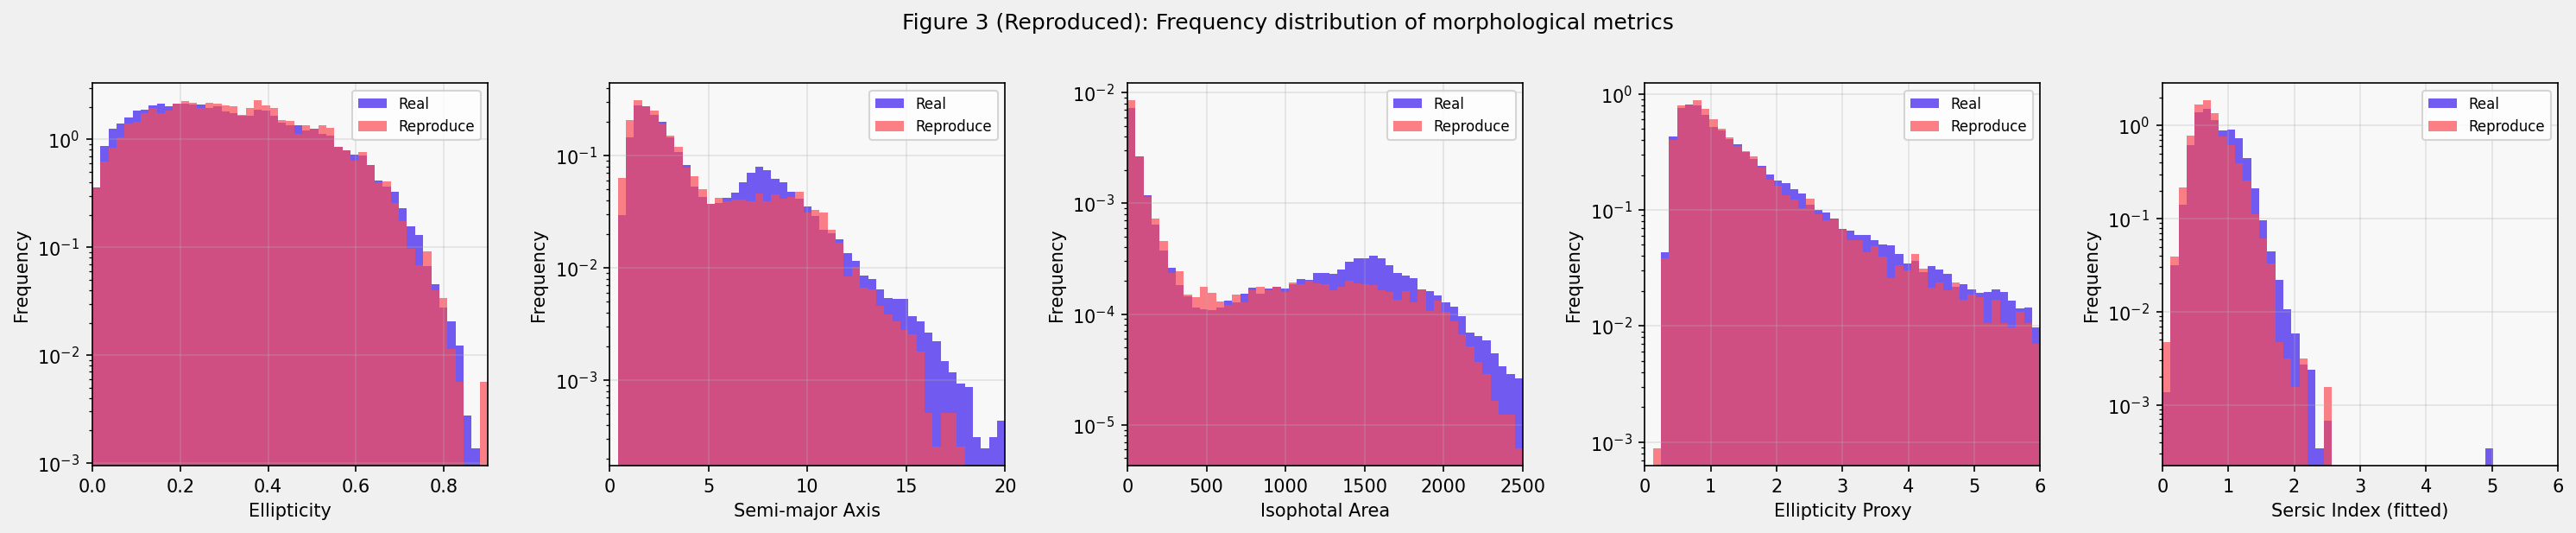
\includegraphics[width=\textwidth]{Metrics/evaluation_result_with_fitted_sersic/figure3_reproduce.png}
    \caption{Morphological metric distributions (two-way comparison): real
    GalaxiesML test images (blue) versus our reproduced DDPM images (red).
    The fitted S\'{e}rsic index (rightmost panel) is an extension not
    present in \citet{lizarraga2024}.}
    \label{fig:morph_reproduce}
\end{figure*}

\begin{figure*}
    \centering
    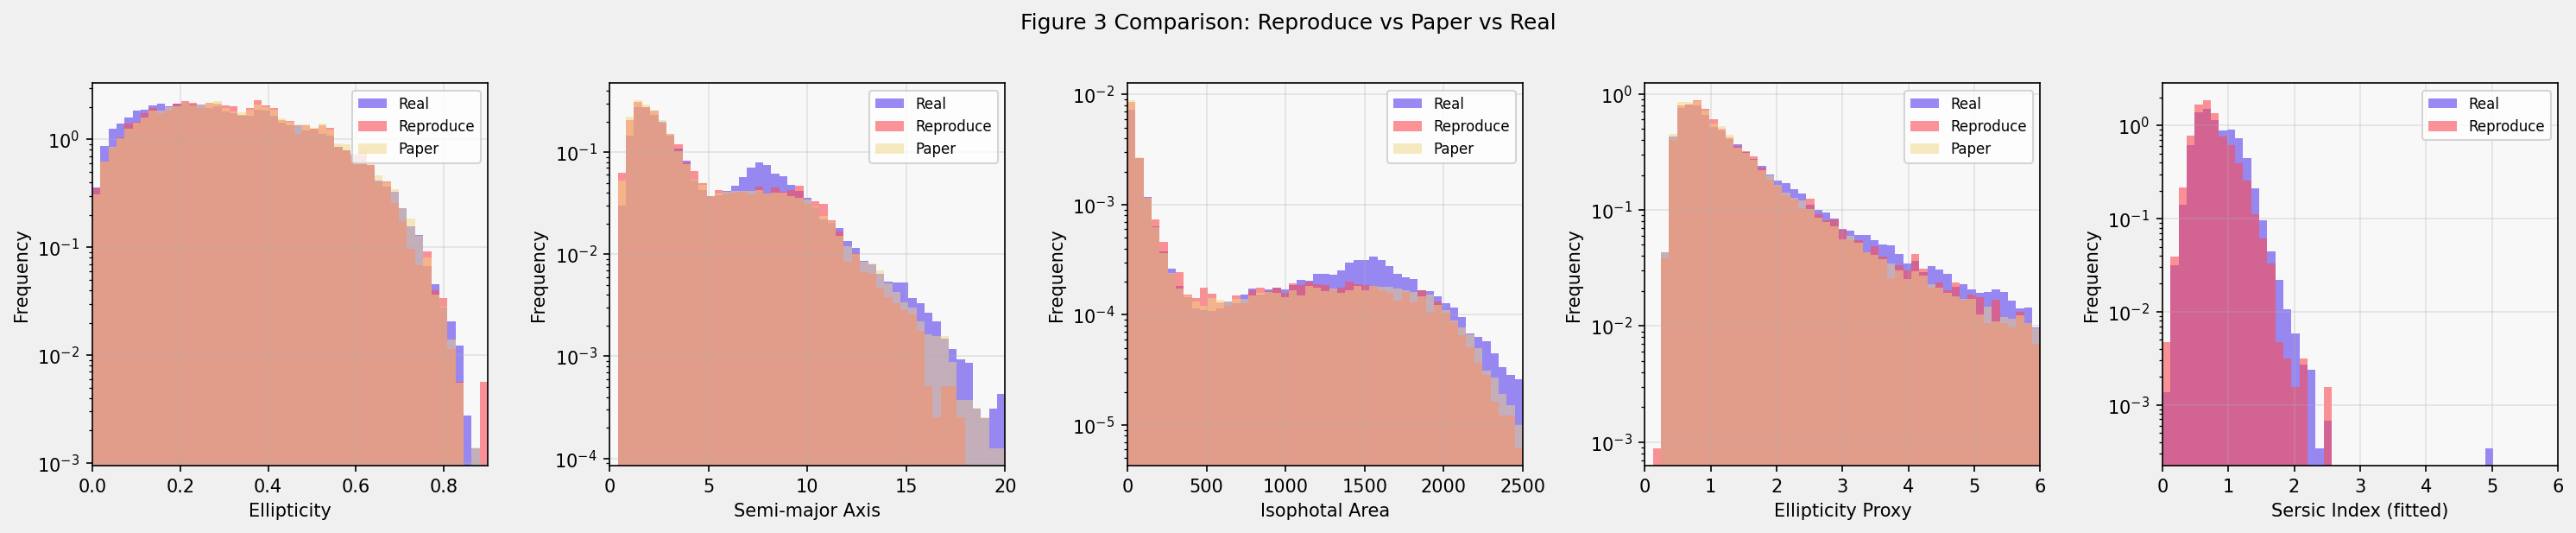
\includegraphics[width=\textwidth]{Metrics/evaluation_result_with_fitted_sersic/figure3_comparison.png}
    \caption{Morphological metric distributions (three-way comparison):
    real GalaxiesML test images (blue), our reproduced DDPM images (red),
    and the original paper's generated images (yellow).}
    \label{fig:morph_comparison}
\end{figure*}

Table~\ref{tab:morph} shows that all Reproduce/Paper ratios within 2 per cent of
unity, confirming a reliable reproduction of \citet{lizarraga2024}. Meanwhile, high paper/real ratio and reproduce/real ratio not only shows the reproduced distributions closely match
the real data, also verifies the accuracy of \citet{lizarraga2024} generation images.

Figure~\ref{fig:morph_redshift} further shows the mean of each metric
as a function of redshift, confirming that the DDPM reproduces not
only the overall distributions but also the correct redshift-dependent
trends.

\begin{figure*}
    \centering
    \includegraphics[width=\textwidth]{Metrics/evaluation_result_with_fitted_sersic/figure4_reproduce_metrics_stats.png}
    \caption{Mean morphological metrics as a function of redshift,
    comparing real GalaxiesML test galaxies (blue) and DDPM-generated
    galaxies (red) across redshift bins.
    Error bars represent 95 per cent confidence intervals on the mean.
    The DDPM accurately reproduces the observed redshift-dependent
    trends in ellipticity, semi-major axis, isophotal area, ellipticity
    proxy, and fitted S\'{e}rsic index.}
    \label{fig:morph_redshift}
\end{figure*}

\begin{table*}
    \centering
    \small
    \caption{Morphological metrics for the GalaxiesML test set and
    generated images.
    $\bar{x}_\mathrm{real}$ is the real test-set mean.
    Paper/Real and Reproduce/Real are the ratios of the generated mean
    to the real mean for \citet{lizarraga2024} and our reproduction
    respectively; a ratio of 1 indicates perfect agreement.
    Reproduce/Paper shows how closely our reproduction matches the
    original paper's generated images.
    All Reproduce/Paper ratios are within 2 per cent of unity,
    confirming a reliable reproduction.
    The fitted S\'{e}rsic index is an extension unique to this work
    and was not computed in \citet{lizarraga2024} (N/A).}
    \label{tab:morph}
    \begin{tabular}{lrrrr}
        \hline
        Metric & $\bar{x}_\mathrm{real}$ & Paper/Real & Reproduce/Real & Reproduce/Paper \\
        \hline
        Ellipticity               & 0.307 & 1.057 & 1.037 & 0.981 \\
        Semi-major axis           & 4.503 & 0.881 & 0.890 & 1.010 \\
        Isophotal area            & 536.3 & 0.759 & 0.757 & 0.998 \\
        Ellipticity proxy         & 2.057 & 0.901 & 0.896 & 0.995 \\
        S\'{e}rsic index (fitted) & 0.837 & N/A   & 0.911 & N/A   \\
        \hline
    \end{tabular}
\end{table*}

%%--------------------------------------------------------------------
\subsection{CNN Redshift Predictor}
\label{sec:cnn_results}

\begin{figure*}
    \centering
    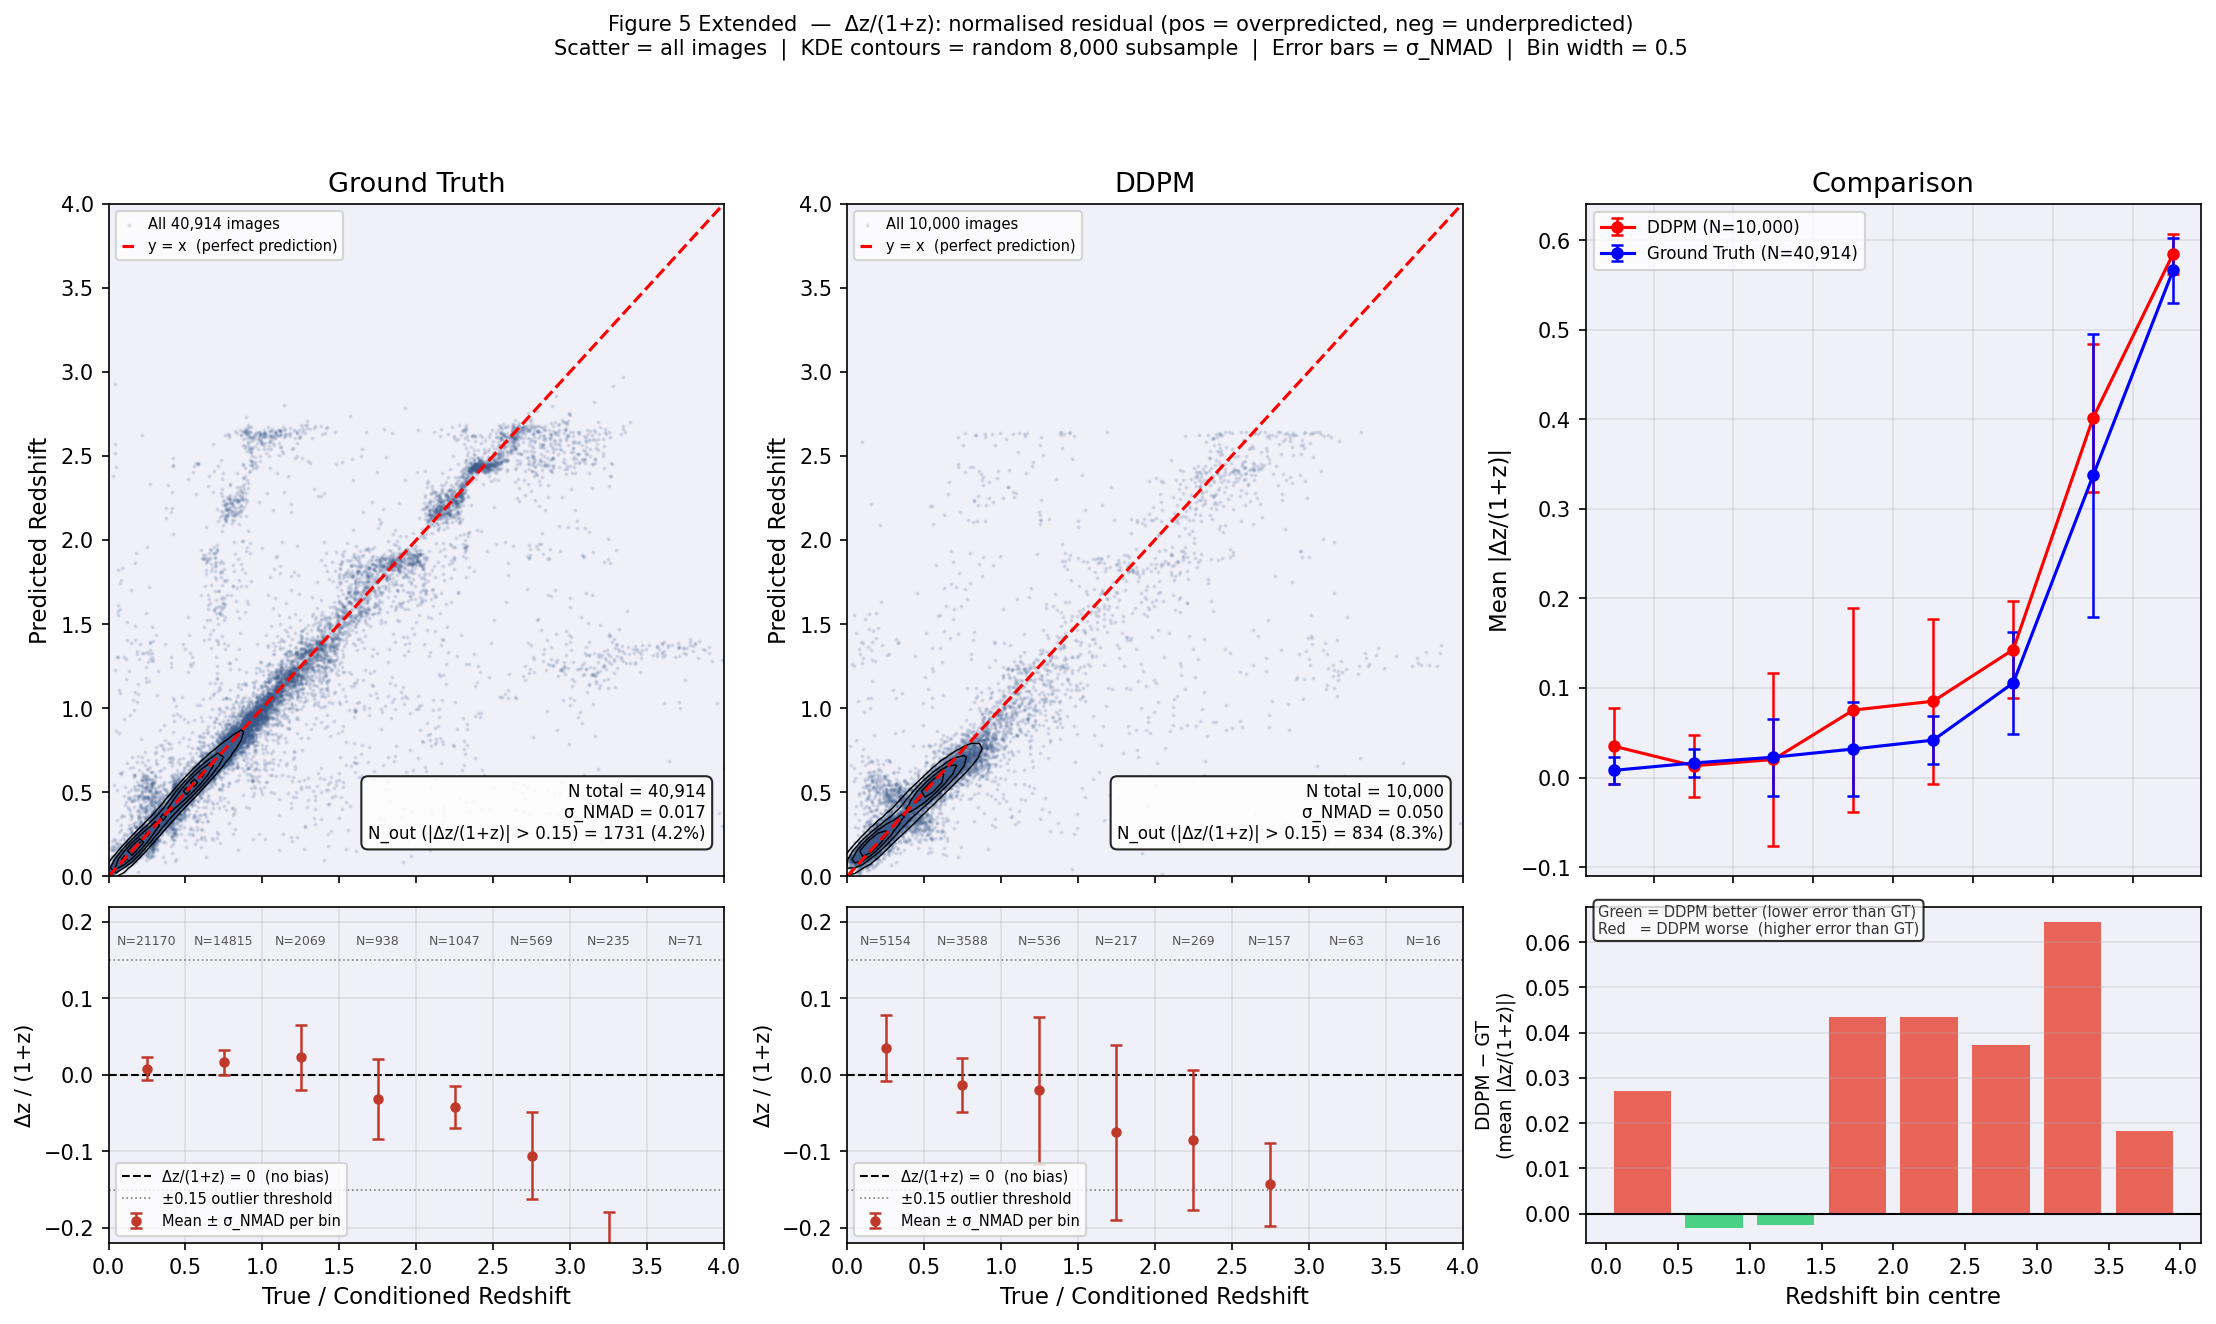
\includegraphics[width=\textwidth]{Metrics/figure5_extended.png}
    \caption{Photo-z scatter plots and residuals, extending Figure~5
    of \citet{lizarraga2024} with an additional bottom row.
    \textit{Top left}: predicted versus true spectroscopic redshift
    for the GalaxiesML test set (ground truth; $N = 40{,}914$;
    $\sigma_\mathrm{NMAD} = 0.017$).
    \textit{Top middle}: predicted versus conditioned redshift for
    DDPM-generated images ($N = 10{,}000$;
    $\sigma_\mathrm{NMAD} = 0.050$).
    \textit{Top right}: mean $|\Delta z/(1+z)|$ per redshift bin
    for real (blue) and generated (red) images.
    \textit{Bottom left and middle}: mean normalised residual
    $\Delta z/(1+z)$ per redshift bin for real and generated images
    respectively.
    \textit{Bottom right}: difference in mean $|\Delta z/(1+z)|$
    between DDPM and ground truth per bin (green = DDPM lower error,
    red = DDPM higher error).}
    \label{fig:cnn_redshift}
\end{figure*}

To verify that the DDPM's redshift conditioning is physically meaningful,
we applied the CNN redshift predictor (Section~\ref{sec:cnn_z}) to
both the GalaxiesML test set and our generated images.
Figure~\ref{fig:cnn_redshift} shows the photo-z scatter plot (predicted
versus true/conditioned redshift) for both sets, reproducing Figure~5
of \citet{lizarraga2024} and extending it with a bottom row of
normalised residuals $\Delta z / (1+z)$ per redshift bin and NMAD (equation~\ref{eq:nmad}) to make systematic biases more explicit.

In both the real and DDPM panels, predictions cluster tightly around
the parity line ($y = x$), confirming that the CNN successfully
recovers the redshift from image features.
On the GalaxiesML test set, the predictor achieves
$\sigma_\mathrm{NMAD} = 0.017$, establishing a strong baseline.
On the DDPM-generated images, $\sigma_\mathrm{NMAD} = 0.050$,
indicating that the conditioned redshift is recoverable with reasonable
accuracy, and confirming that the DDPM has learned physically meaningful
redshift-dependent image features.  Notably, the bottom-right panel of Fig.~\ref{fig:cnn_redshift} shows
that at $z \approx 0.5$--$1.5$, the mean prediction error on DDPM
images is \textit{lower} than on real GalaxiesML galaxies.
This suggests the DDPM generates particularly ``typical'' galaxies images in
this redshift range, and the generated images match the 
appearance of the galaxies that the CNN has learned in each redshift range.


However, this could also indicate reduced diversity in the generated
images: if the DDPM tends to generate very similar images at each
redshift (i.e.\ mode averaging), predictions become easier, but the
generated set may under-represent the true variety of galaxy
morphologies.
This potential lack of diversity is discussed further in
Section~\ref{sec:discussion}.

In addition, two other limitations are visible in the DDPM panel.
First, predictions are more concentrated at low redshift compared to
the real test set, suggesting the model under-generates high-redshift
diversity.
Second, a horizontal stripe is visible near $z \approx 2.7$, indicating
a tendency to predict a fixed low value for some high-redshift inputs.
These issues are discussed further in Section~\ref{sec:discussion}.





















%%--------------------------------------------------------------------
\subsection{MorphCNN: Morphological Parameter Prediction}
\label{sec:morphcnn_results}

\subsubsection{Training}

MorphCNN is trained on the GalaxiesML training set for 22 epochs,
achieving a best validation loss of $3.51 \times 10^{-2}$ under
Huber loss on standardised targets.
The four morphological parameters --- ellipticity, semi-major axis,
S\'{e}rsic index, and isophotal area --- are log-transformed (except
ellipticity) and standardised before training, with the normalisation
statistics saved to allow consistent denormalisation at inference time.

\subsubsection{Performance on the GalaxiesML Test Set}

Figure~\ref{fig:morphcnn_testset} shows the parity plots (predicted
versus true) for all four parameters on the held-out GalaxiesML test
set.
Predictions cluster tightly around the identity line ($y = x$) across
the full dynamic range of each parameter, with high coefficients of
determination ($R^2 = 0.88$, $0.97$, $0.82$, $0.96$ for ellipticity,
semi-major axis, S\'{e}rsic index, and isophotal area respectively)
and low scatter ($\sigma_{\mathrm{NMAD}} = 0.033$, $0.226$, $0.094$,
$27.0$).
The fraction of outliers exceeding 20 per cent relative error is
38.8, 5.1, 11.7, and 12.7 per cent respectively.
These results confirm that MorphCNN learns a reliable mapping from
multi-band galaxy images to morphological parameters.

\begin{figure*}
    \centering
    
\includegraphics[width=0.55\textwidth]{morphCNN/eval_combined_ellipticity.png}\\[4pt]
    
\includegraphics[width=0.55\textwidth]{morphCNN/eval_combined_major_axis.png}\\[4pt]
    
\includegraphics[width=0.55\textwidth]{morphCNN/eval_combined_sersic_index.png}\\[4pt]
    
\includegraphics[width=0.55\textwidth]{morphCNN/eval_combined_isophotal_area.png}
    \caption{MorphCNN evaluation for all four morphological parameters
    (rows: ellipticity, semi-major axis, S\'{e}rsic index, isophotal area).
    \textit{Left}: parity plot (predicted vs.\ true) on the GalaxiesML
    test set with KDE contours.
    \textit{Middle}: parity plot for the DDPM-generated set
    (CNN-predicted vs.\ SEP-measured).
    \textit{Upper right}: mean $|\text{pred} - \text{true}|$ per
    redshift bin for real (blue) and DDPM (red) images.
    \textit{Lower right}: difference in mean absolute error per
    redshift bin (green = DDPM lower error; red = DDPM higher error).}
    \label{fig:morphcnn_testset}
\end{figure*}

\subsubsection{Performance on DDPM-Generated Images}

\begin{figure*}
    \centering
    
\includegraphics[width=\textwidth]{morphCNN/pred_distribution_comparison.png}
    \caption{MorphCNN-predicted distributions for the GalaxiesML test
    set (blue; $N = 40{,}891$) and DDPM-generated images
    (red; $N = 10{,}000$) across all four morphological parameters.
    The predicted distributions match closely.}
    \label{fig:morph_pred_dist}
\end{figure*}

Figure~\ref{fig:morph_pred_dist} shows the MorphCNN-predicted
distributions for both the real test set and the generated images.
The two distributions match closely across all four parameters,
indicating that the model assigns physically plausible morphological
values to generated images.

However, when individual predictions are compared against SEP-measurements of 4 metrics on the DDPM generation set (Fig.~\ref{fig:morphcnn_testset},
middle column), performance degrades substantially relative to the
GalaxiesML test set.
While a positive trend is visible, the scatter is considerably larger:
$\sigma_{\mathrm{NMAD}}$ rises to $0.172$, $1.965$, $0.786$, and
$200.5$ for ellipticity, semi-major axis, S\'{e}rsic index, and
isophotal area respectively, and the fraction of outliers exceeding
20\% climbs to 73--93\%.
The residual panels further reveal a systematic underestimation bias
that grows with true value, particularly for S\'{e}rsic index and
isophotal area.

\subsubsection{Performance gap diagnosis}
\label{sec:performace_gap}

To investigate the origin of this performance gap, we first examine
the CNN encoder's internal representation of the two image sets.
Figure~\ref{fig:tsne} shows a t-SNE projection of the 256-dimensional
feature vectors extracted from the MorphCNN encoder for 1,000 randomly
sampled real and generated images.
The two populations mix together in feature space with no clear
separation, indicating that the CNN does not perceive the two datasets
as structurally different at the level of its learned representations.

\begin{figure}
    \centering
    
\includegraphics[width=\columnwidth]{morphCNN/tsne_features.png}
    \caption{t-SNE projection of 256-dimensional MorphCNN encoder
    features for 1,000 randomly sampled GalaxiesML test images (blue)
    and 1,000 DDPM-generated images (red).
    The two populations mix in feature space with no clear separation,
    representing the CNN encoder does not perceive a significant
    structural difference between the two datasets.}
    \label{fig:tsne}
\end{figure}

Despite the absence of a feature-space domain shift, a clear
photometric difference exists between the two datasets.
Figure~\ref{fig:radial_profile} shows the azimuthally averaged radial
brightness profile in the $g$ band: DDPM-generated galaxies are
systematically fainter than real ones at all radii, while exhibiting
a similar profile slope.
Furthermore, table~\ref{tab:snr} quantifies this using signal-to-noise ratio (SNR).
Across all five photometric bands, the DDPM images have SNR values significantly lower than corresponding real images, with the
greatest deficit in the $g$ and $y$ bands.

\begin{figure}
    \centering
    
\includegraphics[width=\columnwidth]{morphCNN/radial_profile.png}
    \caption{Azimuthally averaged radial brightness profiles in the
    $g$ band for $N = 500$ randomly sampled GalaxiesML test images
    (blue) and DDPM-generated images (red).
    At each radius $r$, the brightness is averaged over all azimuthal
    directions (i.e.\ all pixels at distance $r$ from the galaxy centre),
    collapsing the 2D image to a 1D curve and reducing noise.
    Shaded bands show $\pm 1\sigma$.
    DDPM images are systematically fainter at all radii, while the
    profile slope is similar, indicating a uniform brightness offset
    rather than a structural difference in galaxy morphology.}
    \label{fig:radial_profile}
\end{figure}

\begin{table}
    \centering
    \caption{Signal-to-noise ratio (SNR) comparison between the
    GalaxiesML test set and DDPM-generated images, measured per
    photometric band on 500 randomly sampled images each.
    Signal = mean pixel value within radius $ r< 10$\,px; Noise = standard
    deviation of pixels at radius $r > 25$\,px.
    The DDPM images have consistently lower SNR across all bands.}
    \label{tab:snr}
    \begin{tabular}{lrrrr}
        \hline
        Band &
        \multicolumn{2}{c}{Real SNR} &
        \multicolumn{2}{c}{DDPM SNR} \\
        & mean & median & mean & median \\
        \hline
        $g$ & 16.90 & 7.36 & 10.32 & 5.26 \\
        $r$ & 21.92 & 12.70 & 14.54 & 8.73 \\
        $i$ & 25.51 & 14.82 & 18.99 & 11.36 \\
        $z$ & 20.99 & 13.94 & 14.56 & 9.12 \\
        $y$ & 14.97 & 9.89  &  9.58 & 5.62 \\
        \hline
    \end{tabular}
\end{table}

To test whether this SNR difference causes the MorphCNN performance gap,
we selectively brighten the central region of each generated image.
We define the inner aperture as the circular region within $r < 10$\,px
of the galaxy centre.
For each of 500 randomly sampled real test images, we compute the mean
pixel value within this aperture, and take the median across all images
as the target brightness $\bar{S}_{\mathrm{real}}$.
For each generated image $i$ with inner-aperture mean $\bar{s}_i$, we
then compute a per-image scale factor:
\begin{equation}
    k_i = \mathrm{clip}\!\left(\frac{\bar{S}_{\mathrm{real}}}{\bar{s}_i},\;1,\;5\right),
    \label{eq:brighten_k}
\end{equation}
where the lower bound of 1 ensures we only ever brighten (never darken)
a generated image, and the upper bound of 5 prevents extreme
amplification of images where the galaxy core is near-zero ---
such images would otherwise be scaled by an arbitrarily large factor.
The brightening is then applied via a Gaussian aperture mask
($\sigma = 10$\,px) centred on the galaxy, so that the amplification
is concentrated on the bright central region and the background pixels
are barely affected.
This raises the galaxy core brightness of each generated image to match
the typical brightness of a real galaxy, while leaving the background
largely unaffected.
Unlike a global brightness scaling, which raises signal and noise
equally and leaves SNR unchanged, our brightening approach concentrates the
amplification on the bright central region, increasing SNR.
Table~\ref{tab:brightening} compares $\sigma_{\mathrm{NMAD}}$ before
and after brightening for all four parameters.
Three of the four parameters show a reduction in scatter, with
the largest improvement for isophotal area ($-6.1$ \%),
suggesting that the SNR deficit does contribute to the prediction gap.
However, the improvements are small and the semi-major axis error
slightly increases, indicating that SNR is not the sole cause.

\begin{table}
    \centering
    \caption{$\sigma_{\mathrm{NMAD}}$ comparison between original and
    Gaussian-brightened DDPM images (evaluated against SEP measurements).
    Negative $\Delta$ indicates improvement.
    Three of the four parameters improve after brightening.}
    \label{tab:brightening}
    \begin{tabular}{lrrr}
        \hline
        Parameter & Original & Brightened & $\Delta$ (\%) \\
        \hline
        Ellipticity          & 0.1728 & 0.1715 & $-0.7$ \\
        Major Axis (arcsec)  & 1.9651 & 2.0075 & $+2.2$ \\
        S\'{e}rsic Index $n$ & 0.7863 & 0.7811 & $-0.7$ \\
        Isophotal Area (px$^2$) & 200.5 & 188.3 & $-6.1$ \\
        \hline
    \end{tabular}
\end{table}

The underlying causes of the performance gap are likely multiple and hard to explicitly explore and explain. They
may include model learning reasons, differences in the pixel intensity distribution, and other
dataset-level differences between the real and generated sets.
We discuss further in Section~\ref{sec:discussion}.

%%--------------------------------------------------------------------
\subsection{Redshift Label Perturbation $\sigma$ and FID}
\label{sec:sigma_ablation}

The redshift label perturbation $\sigma$ (equation~\ref{eq:label_smooth})
controls how much Gaussian noise is added to the conditioning redshift
during training.
We train DDPM models at $\sigma \in \{0.01,\, 0.1,\, 0.5,\, 1.0\}$
to investigate its effect on generation quality as measured by FID,
and adopt $\sigma = 0.01$ as our default based on the results.

Table~\ref{tab:sigma_fid} summarises the training outcomes and FID
scores for each configuration.
All four models converged successfully.

The results reveal a clear monotonic trend: smaller $\sigma$ yields
lower FID, with scores decreasing from $24.0$ at $\sigma = 1.0$ to
$15.2$ at $\sigma = 0.5$, $14.2$ at $\sigma = 0.1$, and $4.96$ at
$\sigma = 0.01$.
This suggests that less perturbation of the conditioning redshift
during training allows the model to learn a sharper, more faithful
mapping from redshift to galaxy morphology, resulting in higher
fidelity generated images.
In other words, the DDPM benefits from receiving a precise redshift
signal rather than a smoothed one. This is consistent with the
intuition introduced in Section~\ref{sec:label_smooth}: as the label
perturbation decreases, the conditioning signal becomes sharper, and
the model can more easily distinguish fine-grained morphological
differences between different redshifts.

\begin{table}
    \centering
    \caption{DDPM models trained at different redshift label
    perturbation strengths $\sigma$, with training outcomes and FID
    scores (lower FID is better).
    The FID for $\sigma = 0.01$ is our own evaluation on 10,000
    generated images against the GalaxiesML test set.
    FID values marked $^\dagger$ are taken from \citet{lizarraga2024},
    as our own evaluation could not be completed due to CSD3 cluster
    downtime; the corresponding training runs completed successfully.}
    \label{tab:sigma_fid}
    \begin{tabular}{cccc}
        \hline
        $\sigma$ & Stopped at epoch & Val loss & FID \\
        \hline
        0.01 & ---  & ---    & 4.96 \\
        0.1  & 261  & 0.0005 & $14.2^\dagger$ \\
        0.5  & 145  & 0.0008 & $15.2^\dagger$ \\
        1.0  & 263  & 0.0005 & $24.0^\dagger$ \\
        \hline
        \multicolumn{4}{l}{$^\dagger$ FID from \citet{lizarraga2024}.}
    \end{tabular}
\end{table}

\clearpage
\section{Discussion}
\label{sec:discussion}

%%--------------------------------------------------------------------
\subsection{What the Reproduction Confirmed}

Our reproduction of \citet{lizarraga2024} confirms the core finding
that a redshift-conditioned DDPM can generate physically realistic
galaxy images.
The morphological metric distributions of our generated images match
those of the original paper to within 2\%(Table~\ref{tab:morph}),
and both reproduce the qualitative redshift-dependent trends seen in
the real GalaxiesML test set (Fig.~\ref{fig:morph_redshift}).
The photo-z scatter plot (Fig.~\ref{fig:cnn_redshift}) further
confirms that the DDPM has learned a meaningful mapping from redshift
to visual appearance: an independent CNN trained only on real galaxies
can recover the conditioned redshift of generated images with
$\sigma_\mathrm{NMAD} = 0.050$.

%%--------------------------------------------------------------------
\subsection{Problems Revealed}

\subsubsection
{S\'{e}rsic index}

We found that the ``S\'{e}rsic index'' reported in
\citet{lizarraga2024} is not a fitted profile parameter but an
ellipticity-based proxy (equation~\ref{eq:proxy_sep}), a heuristic
approximation that does not involve radial brightness profile
fitting.
We replace this with a proper fitted S\'{e}rsic index in our
evaluation (Section~\ref{sec:sersic}).

\subsubsection
{Measurement Method Mismatch Between SEP and HSC Pipeline}
\label{sec: HSC_vs_SEP}

\begin{figure*}
    \centering
    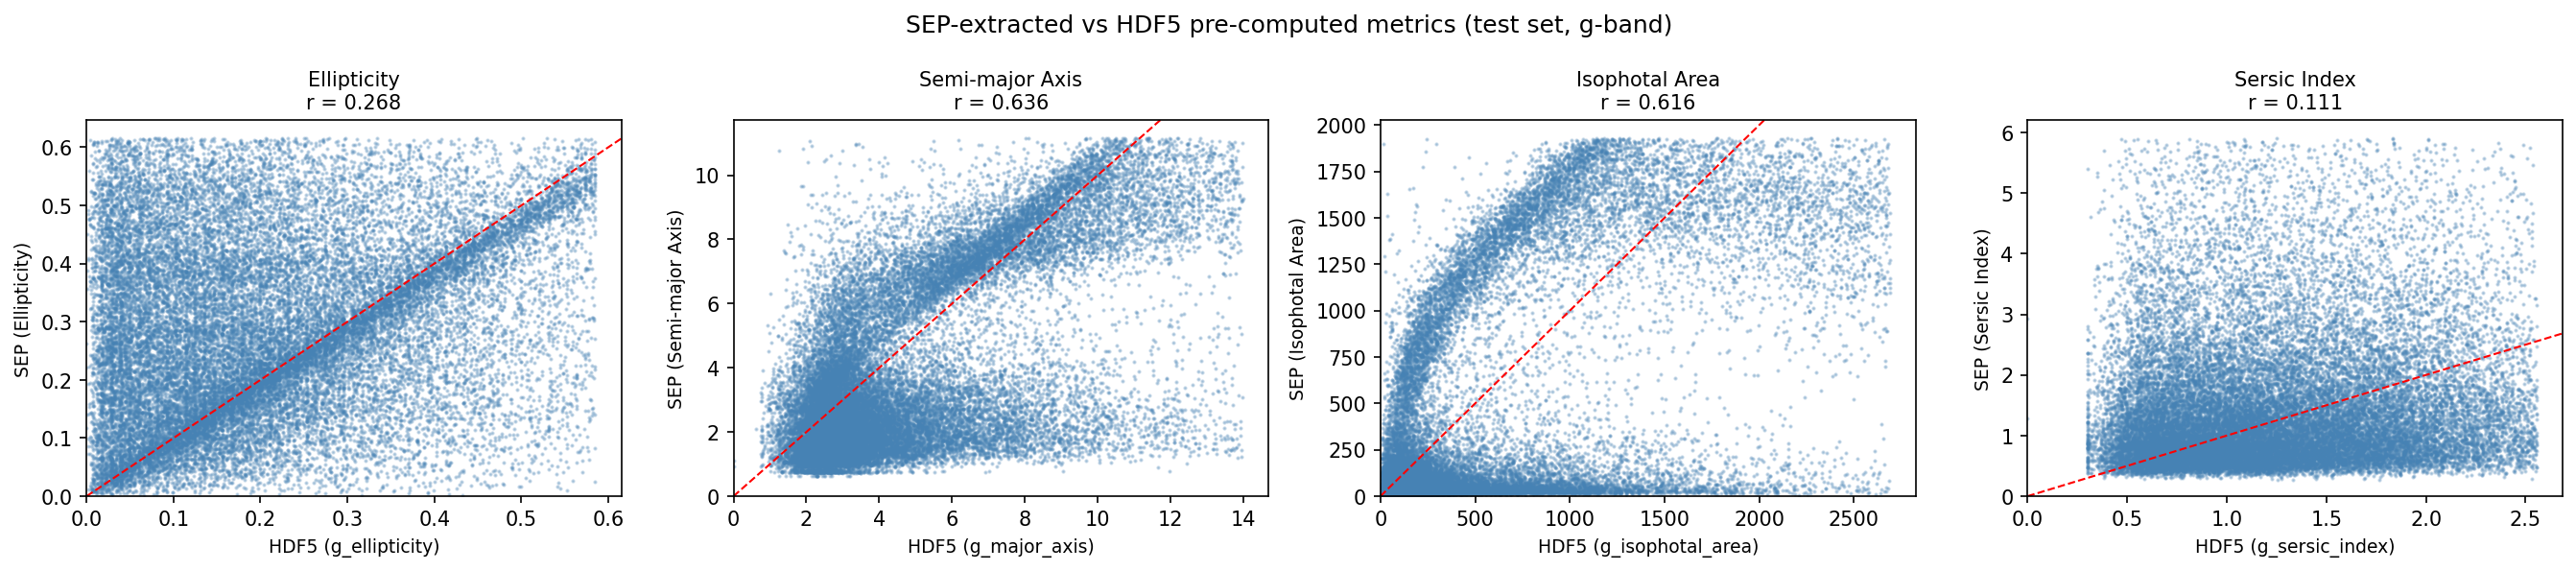
\includegraphics[width=\textwidth]{Metrics/compare_sep_vs_hdf5.png}
    \caption{Per-galaxy comparison of SEP-extracted metrics
    (vertical axis) versus HSC pre-computed catalogue values
    (horizontal axis) for the GalaxiesML test set, measured in
    the $g$ band.
    The S\'{e}rsic index shown is our fitted value from isophote
    profile fitting (Section~\ref{sec:sersic}), not the ellipticity
    proxy.
    Pearson correlation coefficients are shown for each metric.
    The moderate correlation for the fitted S\'{e}rsic index
    ($r = 0.405$) reflects methodological differences between our
    isophote-based 1D profile fit and the HSC pipeline's approach,
    despite both using profile fitting.}
    \label{fig:sep_vs_hsc}
\end{figure*}

\begin{figure*}
    \centering
    
\includegraphics[width=\textwidth]{Metrics/evaluation_fitted_sersic_with_repo_tes/figure3_paper_real.png}
    \caption{Morphological metric distributions when HSC catalogue
    values are used for real galaxies (blue) rather than SEP
    re-extracted values.
    \textit{Above}: comparison between HSC catalogue metrics (real)
    and SEP-extracted metrics (reproduced DDPM).
    \textit{Below}: three-way comparison additionally including the
    original paper's generated images.
    The distribution mismatches become apparent due to the measurement
    method difference.}
    \label{fig:sep_vs_hsc_dist}
\end{figure*}

The GalaxiesML dataset provides pre-computed morphological parameters
measured by the HSC photometric pipeline.
Although the HSC pipeline also uses \textsc{SExtractor} internally,
it applies a different configuration, including different detection
thresholds, deblending parameters, and aperture definitions. Since the configuration is unknown, we cannot reproduce and apply it to our DDPM-generated
images.
To ensure a fair comparison, we therefore re-extracted all four
metrics from the GalaxyML test set images using our own \textsc{sep}
configuration, identical to what we applied to the generated images.

However, this re-extraction introduces a systematic offset between
the SEP-measured values and the HSC catalogue values.
Figure~\ref{fig:sep_vs_hsc} shows the correlation between
the two measurement methods on the GalaxyML test set.
Pearson correlation coefficients range from $r = 0.250$ for
ellipticity to $r = 0.635$ for semi-major axis.
The fitted S\'{e}rsic index achieves a moderate correlation of
$r = 0.405$, despite both methods using profile fitting; the
remaining scatter reflects differences in the specific fitting
procedure, isophote extraction, and sky-subtraction between
our SEP-based pipeline and the HSC approach.

As a consequence, if one were to compare our generated-image metrics
(measured with SEP) against the HSC catalogue values for real images,
apparent distribution mismatches would arise from this
methodological difference rather than from any failure of the DDPM.
Figure~\ref{fig:sep_vs_hsc_dist} illustrates this: using HSC
catalogue values for GalaxyML test set alongside SEP values for generated
galaxies produces visibly different distributions, even though the
underlying images are the same.
This is a difficulty in galaxy morphology studies:  different
measurement pipelines produce different parameters, and we can not know which one is correct or the best. This motivates our choice to re-extract all metrics with a single
consistent tool.

\subsubsection{CNN Redshift Predictor Bias Towards Low Redshift}

\begin{figure}
    \centering
    \includegraphics[width=\columnwidth]{ddpm/dataset_redshift_distribution.png}
    \caption{Redshift distribution of the GalaxiesML training set.
    The dataset is strongly skewed towards low redshift, with the
    majority of galaxies at $z < 1$.
    High-redshift galaxies ($z > 2$) are sparsely represented,
    which biases both the CNN predictor and the DDPM towards
    low-redshift features.}
    \label{fig:redshift_dist}
\end{figure}

As noted in Section~\ref{sec:cnn_results}, the CNN predictor
over-predicts at low redshift for the generated images.
Moreover, the mean $|\Delta z/(1+z)|$ increases monotonically with
redshift (Fig.~\ref{fig:cnn_redshift}, top right), indicating that
prediction uncertainty grows with $z$ and the model becomes
progressively less reliable at high redshift.
A horizontal stripe at $z \approx 2.7$ further suggests that the
model collapses to a fixed prediction for some high-redshift inputs.

Both effects are rooted in the GalaxiesML training data distribution
(Fig.~\ref{fig:redshift_dist}): the dataset is strongly dominated by
low-redshift galaxies, with very few examples at $z > 2$.
As a result, the CNN predictor is biased towards the dominant
low-$z$ class and has seen too few high-$z$ examples to learn
reliable features at those redshifts.
The DDPM is trained on the same imbalanced distribution, so its
generated images at high redshift may not faithfully reflect the
true diversity of high-$z$ morphologies, further compounding the
predictor bias.



\subsubsection{MorphCNN performance gap reflection}


A plausible explanation for the systematic brightness deficit and SNR difference reflected in ~\ref{sec:performace_gap} lies in
how diffusion models learn the training data distribution.
Galaxy images are dominated by dark background pixels: the bright
galaxy core occupies only a small fraction of the $64 \times 64$
image, while the vast majority of pixels contain sky background at
near-zero flux.
The DDPM is therefore trained on a pixel distribution that is
heavily skewed towards low values.
During generation, the model implicitly averages over this
distribution, which is a phenomenon known as \textbf{regression to the mean}, producing images in which the galaxy core is systematically
underexposed relative to real HSC observations. As a result, the generated images are darker than the images in GalaxyML test set.
This is a limitation of diffusion models on datasets with
highly imbalanced pixel distributions, and is not specific to galaxy
imaging.

A further source of the performance gap is a label inconsistency
between training and evaluation.
MorphCNN was trained on the HSC photometric catalogue values
stored
in the GalaxiesML dataset, which were derived from the HSC
pipeline.
When evaluating on DDPM-generated images, we obtained the "ground truth" by
running SEP on each generated image.
As demonstrated in Section~\ref{sec: HSC_vs_SEP}, the HSC pipeline
and SEP do not produce equivalent measurements for the same galaxy, so the model
is effectively being compared against a different measurement system
to the one it was trained on.
Retraining MorphCNN on SEP-extracted labels for the full
204,573-image training set would eliminate this inconsistency, but
this task could not be completed due to unexpected downtime of the
CSD3 HPC cluster.

%%--------------------------------------------------------------------
\subsection{Limitations and Future Work}

\subsubsection{Compute Interruptions on CSD3}

Most training, evaluation, and generation tasks were conducted on
the CSD3 HPC cluster.
However, several jobs were interrupted mid-run by unexpected cluster
downtime, leaving key tasks incomplete.
Specifically, the FID evaluation for the $\sigma \in \{0.1, 0.5, 1.0\}$
ablation models (Section~\ref{sec:sigma_ablation}) was terminated
before completion. Also, the SEP metric extraction across the full
204,573-image GalaxiesML training set was also terminated, which would have enabled
retraining MorphCNN on consistent SEP-based labels
Section~\ref{sec:morphcnn_results}.
Other planned experiments also could not be completed within the available compute window.



\subsubsection{High-Redshift Data Sparsity and Single-Band Metric Extraction}

A fundamental limitation of this work is the severe class imbalance in the
GalaxiesML dataset (Fig.~\ref{fig:redshift_dist}).
Because high-redshift galaxies ($z > 2$) are sparsely represented
in both the training and test sets, neither the DDPM nor the CNN
predictor can be adequately evaluated at high redshift.
Future work could address this by applying redshift-stratified
sampling or augmentation strategies during training to balance
the class distribution.

\subsubsection{Single-Band Metric Extraction and Multi-Band Conditioning}

A further limitation concerns how the five HSC bands are used.
Although the DDPM and MorphCNN both take all five bands as input,
the SEP-based evaluation metrics (ellipticity, semi-major axis,
S\'{e}rsic index, and isophotal area) are extracted from the $g$
band only, discarding the morphological information encoded in the
remaining four bands.
Similarly, the visual comparisons render the five-band images as
three-channel RGB composites (mapping $i \to R$, $r \to G$,
$g \to B$), omitting the $z$ and $y$ bands entirely.
These choices are common in astrophysics and save computing resources, but discard potentially useful signal,
and future work should extract metrics from all five bands
independently.

More fundamentally, the current DDPM is conditioned only on
redshift.
This work shows that a CNN predictor can successfully back-predict
redshift from generated images precisely compared than the MorphCNN. One of the reasons is that redshift is the
conditioning variable, so the model is explicitly trained to embed
redshift information into the generated images.
By the same logic, MorphCNN struggles to recover morphological
parameters from generated images because those parameters were
never part of the conditioning signal.
A natural extension would be to train a DDPM conditioned jointly
on redshift \textit{and} morphological parameters (e.g.\ ellipticity,
S\'{e}rsic index), analogously to how text-to-image diffusion models
accept multiple conditioning inputs.
Such a model would allow controlled generation of galaxies with
specified morphologies, and would provide a stronger test of whether
the diffusion model has truly learned the relationship between
physical parameters and visual appearance.

\section{Conclusions}

We reproduced the redshift-conditioned DDPM of \citet{lizarraga2024}
and confirmed its core findings.
The DDPM successfully learns to generate physically realistic galaxy
images conditioned on redshift, reproducing observed morphological
distributions and colour evolution trends.
The CNN redshift predictor further confirms this: an independent model
trained only on real galaxies can recover the conditioned redshift of
generated images with reasonable accuracy, demonstrating that the
generated images carry meaningful physical information.

We introduced several extensions.
First, we fit a proper S\'{e}rsic index to replace the original
ellipticity proxy.
Second, we propose MorphCNN, a residual CNN for predicting four
morphological parameters (ellipticity, semi-major axis, S\'{e}rsic
index, and isophotal area) directly from galaxy images.
Third, we also introduced new training strategies, including early stopping and a
learning rate scheduler, to improve DDPM training efficiency.
Finally, we provide several analytical improvements, including per-bin
residual analysis of CNN redshift predictions, colour evolution
analysis of generated samples, and a systematic comparison of
different morphological measurement approaches including the effect
of redshift label perturbation $\sigma$ on generation quality.

Several problems were also identified.
SEP and the HSC pipeline produce systematically different measurements
for the same galaxies, and this mismatch must be accounted for in any
fair comparison between generated and real images.
MorphCNN performs substantially worse on generated images than on real
ones.
We attribute this to a systematic brightness deficit in generated
images (regression to the mean) and a label inconsistency between the
measurement systems used for training and evaluation.

Future work should address high-redshift data sparsity through
redshift-stratified sampling, extend metric extraction to all five HSC
bands, and explore conditioning the DDPM jointly on redshift and
morphological parameters to enable controlled galaxy generation.

\section*{Acknowledgements}

The author thanks Dr.\ Sandro Tacchella for supervision and guidance
throughout this project.

%%%%%%%%%%%%%%%%%%%%%%%%%%%%%%%%%%%%%%%%%%%%%%%%%%
\section*{Data Availability}

 
The GalaxiesML dataset used in this work is publicly available on
Zenodo at \url{https://zenodo.org/records/11117528}.




%%%%%%%%%%%%%%%%%%%% REFERENCES %%%%%%%%%%%%%%%%%%

% The best way to enter references is to use BibTeX:

\bibliographystyle{mnras}
\bibliography{references}


% Alternatively you could enter them by hand, like this:
% This method is tedious and prone to error if you have lots of references
%\begin{thebibliography}{99}
%\bibitem[\protect\citeauthoryear{Author}{2012}]{Author2012}
%Author A.~N., 2013, Journal of Improbable Astronomy, 1, 1
%\bibitem[\protect\citeauthoryear{Others}{2013}]{Others2013}
%Others S., 2012, Journal of Interesting Stuff, 17, 198
%\end{thebibliography}

%%%%%%%%%%%%%%%%%%%%%%%%%%%%%%%%%%%%%%%%%%%%%%%%%%

%%%%%%%%%%%%%%%%% APPENDICES %%%%%%%%%%%%%%%%%%%%%

% Don't change these lines
\bsp	% typesetting comment
\label{lastpage}
\end{document}

% End of mnras_template.tex
